\documentclass{article}
\usepackage[paper=a4paper,margin=0.5in]{geometry}
\usepackage{hyperref}
\usepackage{gensymb}
\usepackage{graphicx}
\usepackage{booktabs}
\usepackage{fancyvrb}
\usepackage{xcolor}
\usepackage{listings}
\usepackage{xparse}
\usepackage{amsmath}
\lstset { %
	language=C++,
	backgroundcolor=\color{blue!5}, % set backgroundcolor
	basicstyle=\footnotesize,% basic font setting
}

\lstset{
	frame=tb, % draw a frame at the top and bottom of the code block
	tabsize=4, % tab space width
	showstringspaces=false, % don't mark spaces in strings
	numbers=left, % display line numbers on the left
	commentstyle=\color{green}, % comment color
	keywordstyle=\color{blue}, % keyword color
	stringstyle=\color{red} % string color
}

\NewDocumentCommand{\codeword}{v}{%
	\texttt{\textcolor{blue}{#1}}%
}
\begin{document}
	\null\hfill\begin{tabular}[t]{l@{}}
	\textbf{Michael Dallas Griffith} \\
	\textit{Final Project Write Up} \\
	\textit{CSCI 551}\\
	\end{tabular} \\ \\
\section*{Riemann Sum Integration Estimation}
\subsubsection*{Using OpenMP, MPI, and Pthreads}
\subsection*{Overview}
For my final project for CSCI 551 -- Parallel and Numerical programming I chose to look at the performance and efficacy of multiple different parallel options to approach a Riemann sum integration estimation.
\subsection*{Riemann Sum}
For the sake of this project, I chose to implement a trapezoidal Riemann sum method. The implementation is to find the area underneath the curve between some point $x$ and some point $x+dx$ and assume that the curve creates a perfect trapezoid. With a sufficiently small $dx$, we can get pretty accurate estimation of a function.
\subsection*{Implementations and Assumptions}
\begin{itemize}
	\item For ease of use within testing, I chose to utilize the function $f(x)=sin(x)$, calculating the definite integral $\int_{0}^{\pi}sin(x)dx$. This allows me to figure out how accurate my results are for the programs easily, but my code is extensible to any function $f(x)$.
	\item I chose $dx = 1\times10^{-8}$ because it is an amply small enough step size that will cause the code to run for a physically tangible amount of time. Any smaller will cause such a large slowdown in functionality that it would be impractical to test on the systems I have. Much larger would have had a less significant speedup due to parallelization.
	\item For the sake of not having to sufficiently concern over floating point precision, I used \codeword{long double}. The code is drafted using a template, so we could easily change the type in the makefile if we wanted to test the precision of different types.
	\item All methods implementing a single method of parallel is done on my personal system. My computer is using an Intel i5-7200U with 4 dedicated cores with hyperthreading enabled. None of the programs that I am running have any memory or I/O intensity to them, so I am purely measuring CPU performance with these methods.
\end{itemize}
\subsection*{Value Results}
\subsubsection*{OpenMP Min/Max/Average Values}
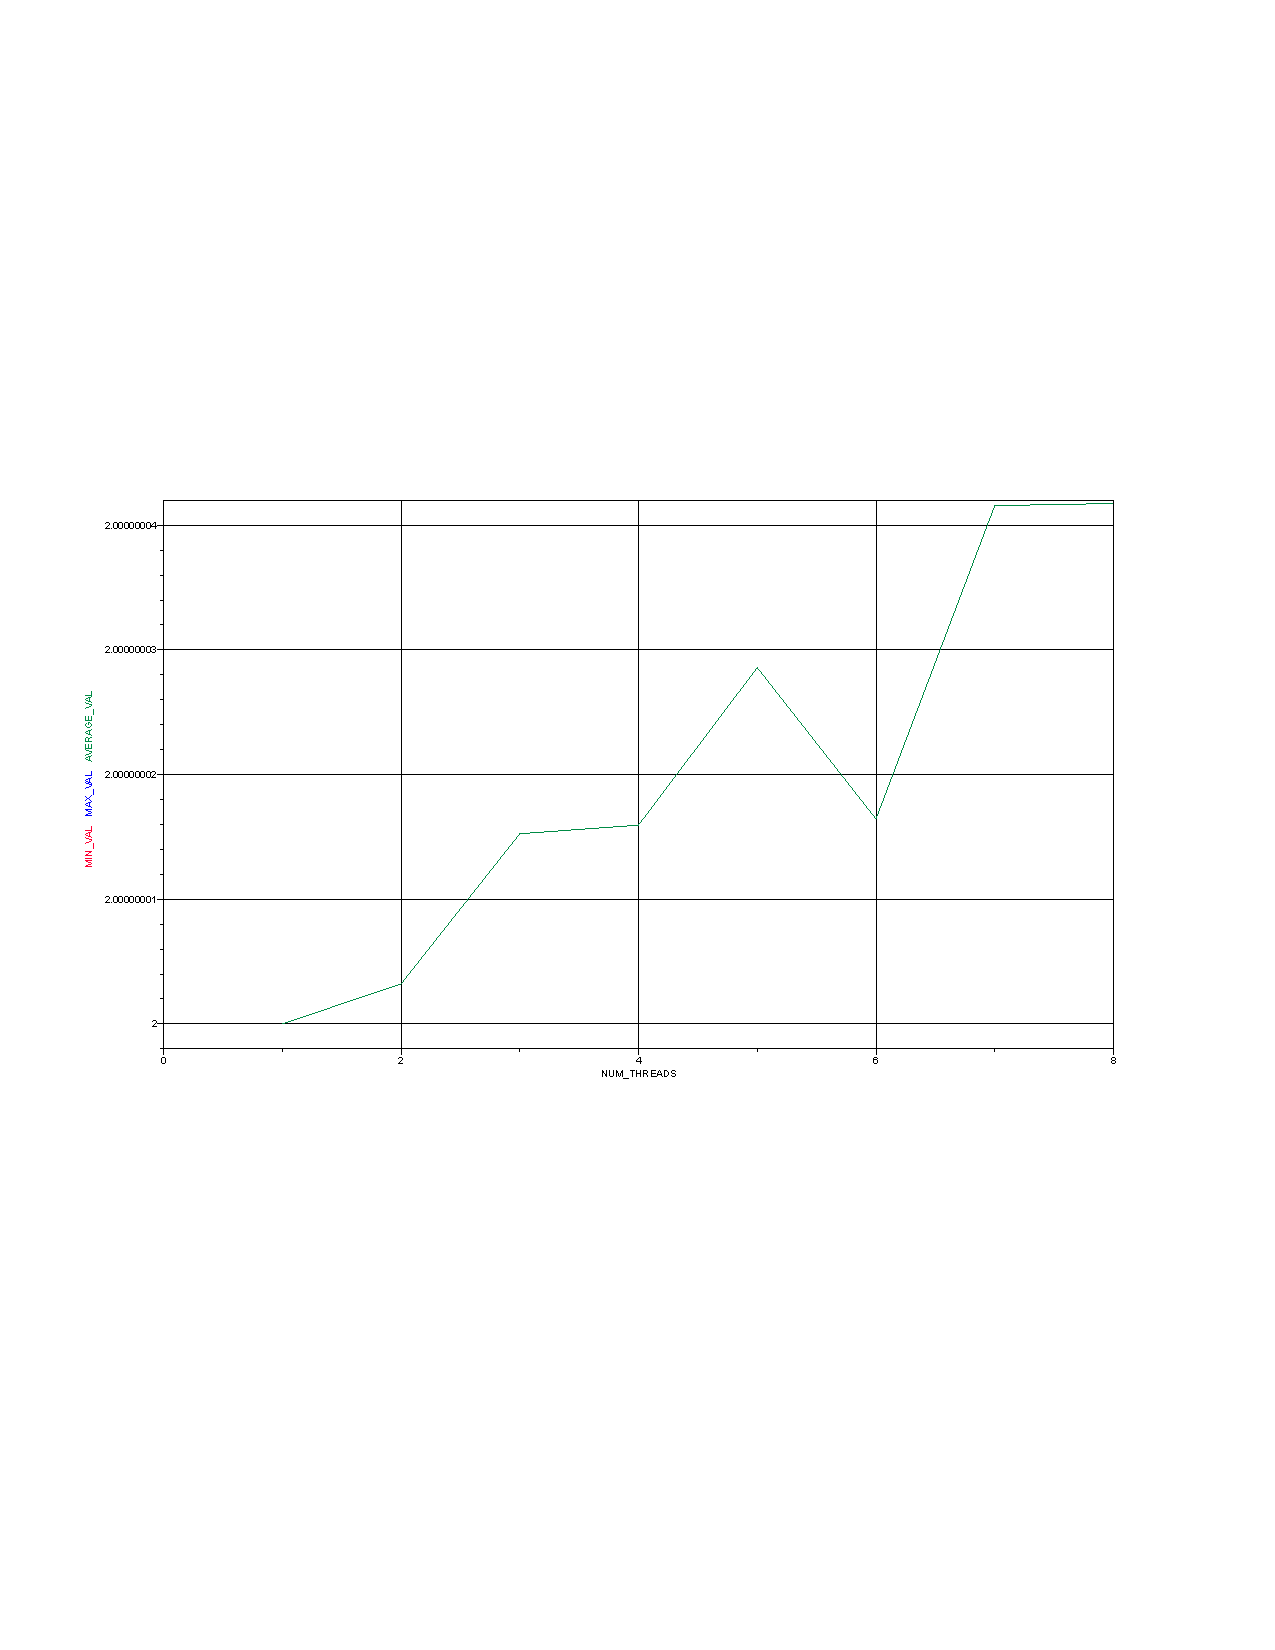
\includegraphics[scale=0.5]{images/omp_vals.pdf}
\subsubsection*{Pthread Min/Max/Average Values}
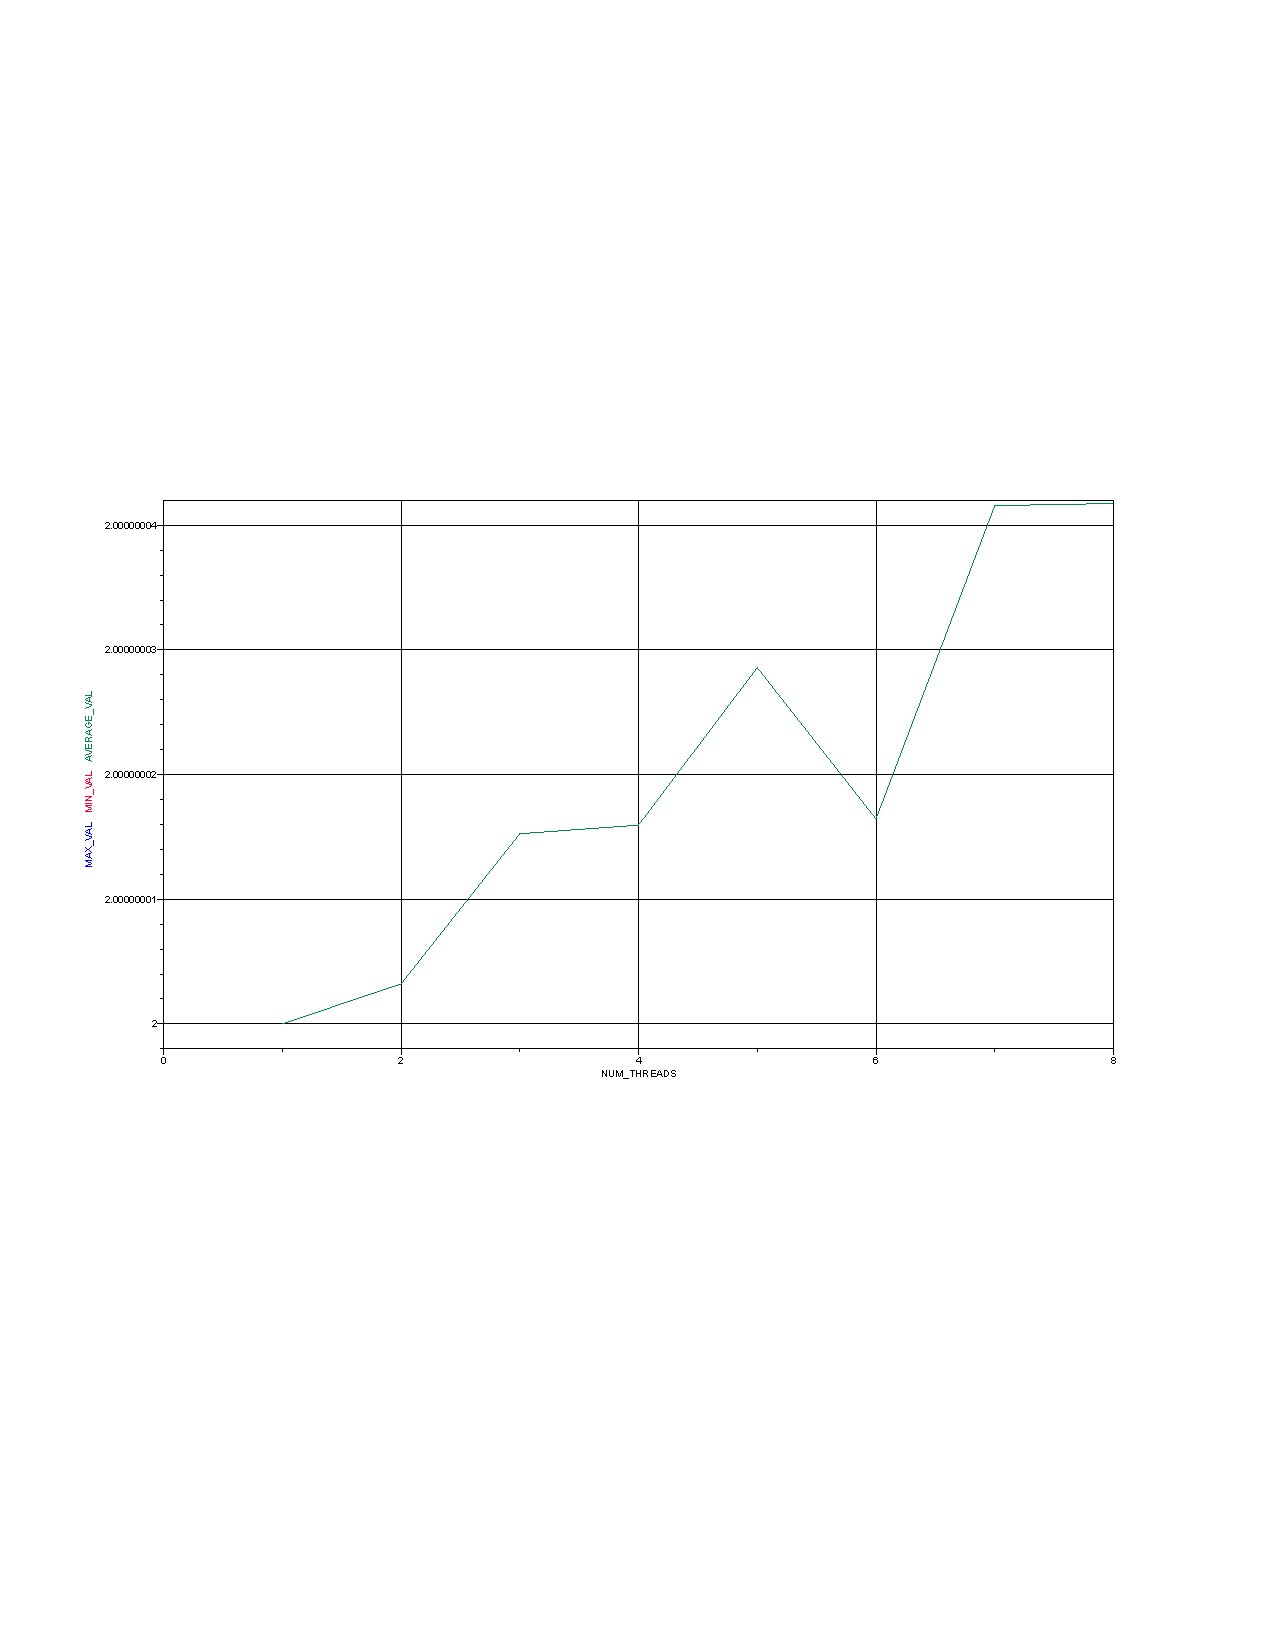
\includegraphics[scale=0.5]{images/pthread_vals.pdf}
\subsubsection*{MPI Min/Max/Average Values}
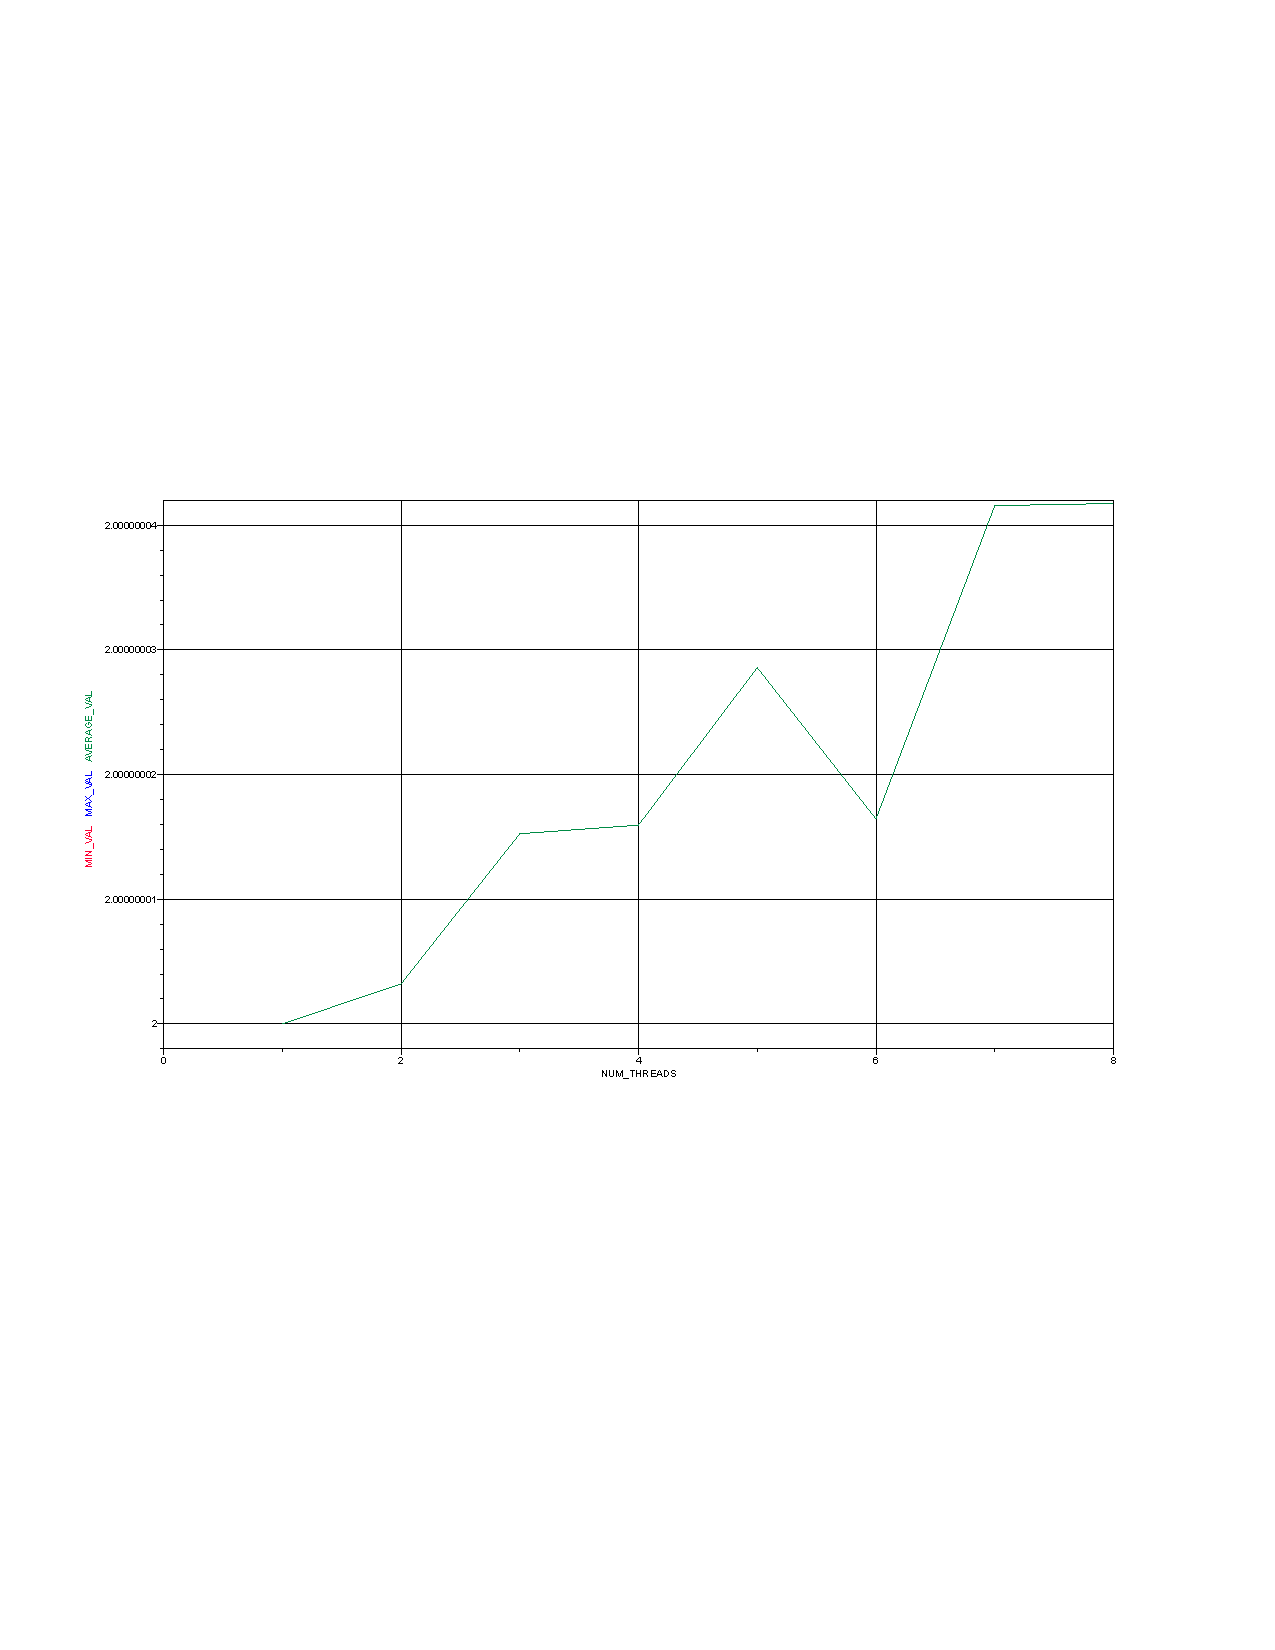
\includegraphics[scale=0.5]{images/mpi_vals.pdf}\\
Attached are small thumbnails of graphs generated by my code that represent the minimum, maximum, and average values as we increase our threads/processes for each parallel implementation. All of these values are generated by 10 runs at each number of threads/processes to gain these statistics. It may be difficult to see from the graphs, but the attached csv should be able to show you that over the course of 10 runs, we attained the exact same results, and the only fluctuation in accuracy was due to adding additional threads. The fluctuation is only on the scale of 0.00000004 seconds, so for the sake of this conversation, we will consider the program to be "sufficiently accurate"
\subsection*{Time Results}
\subsubsection*{OpenMP Min/Max/Average Times per Thread}
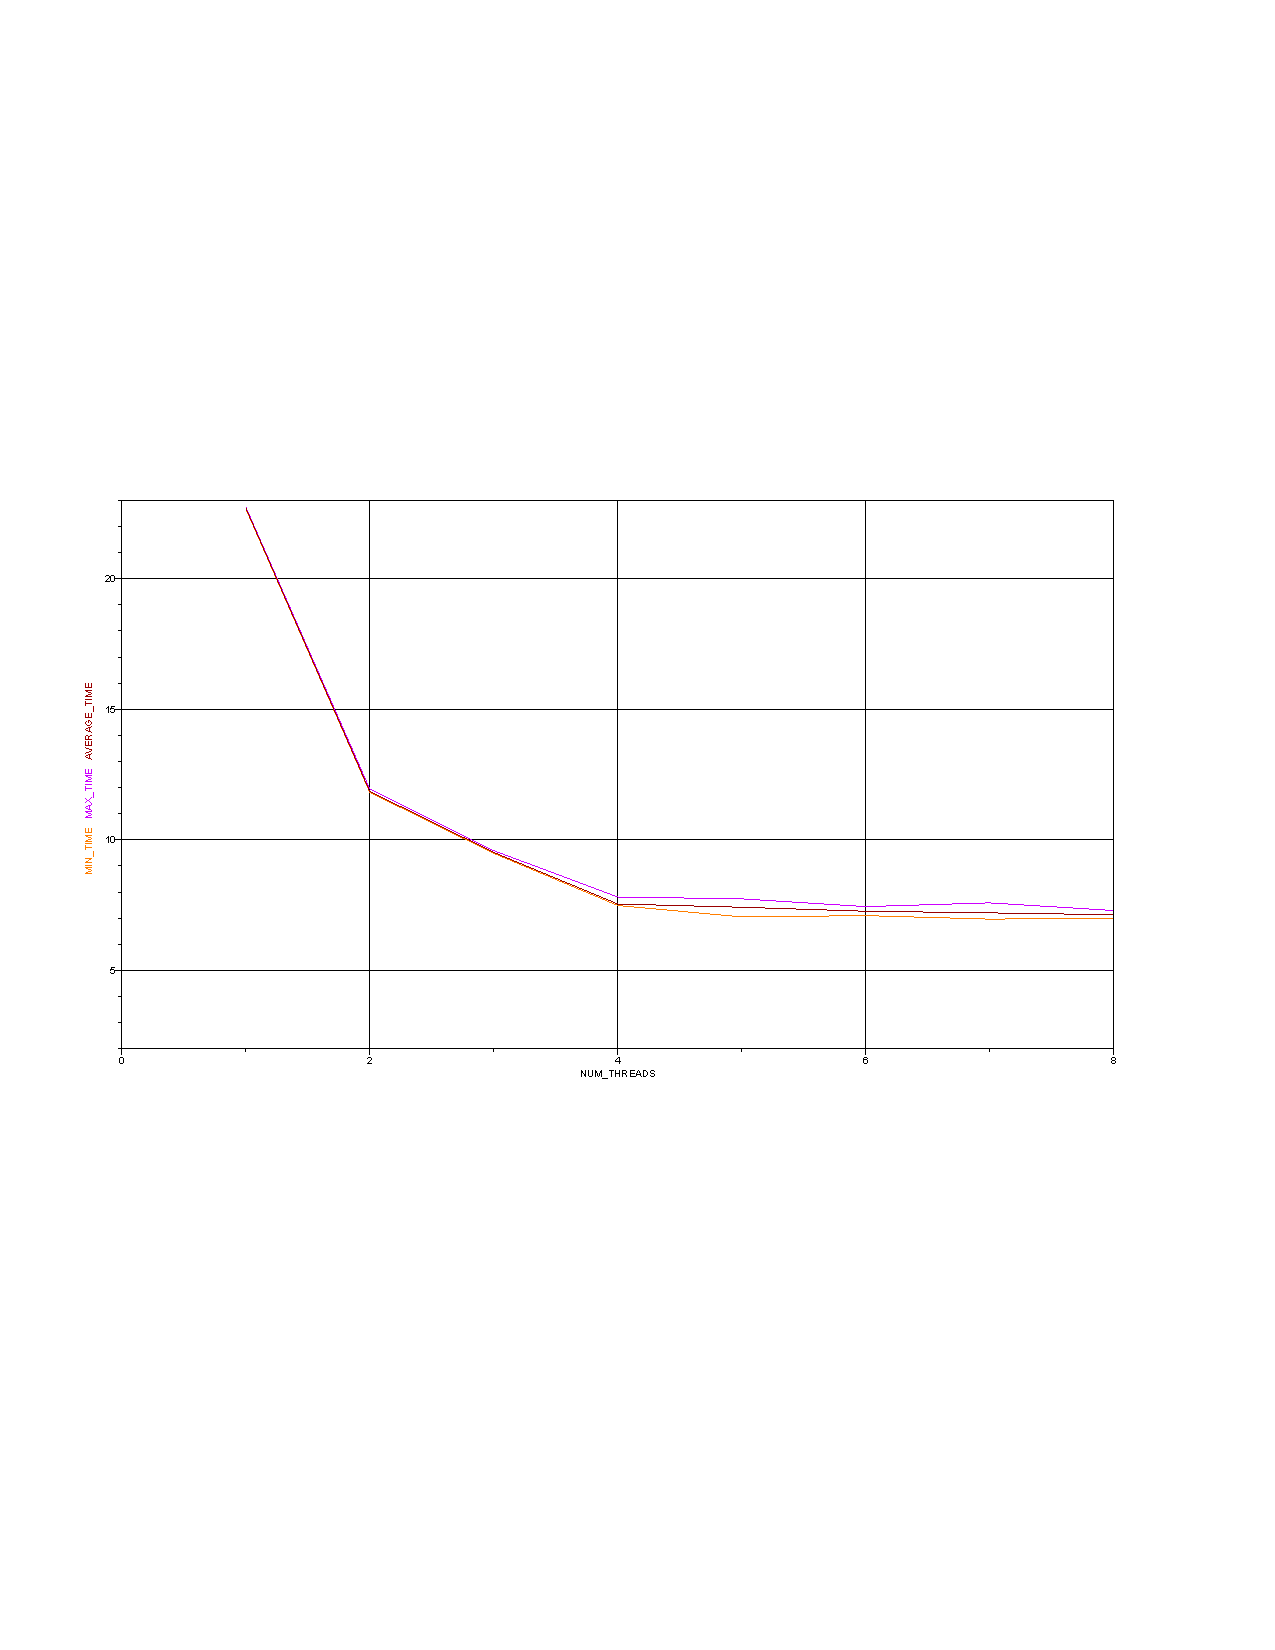
\includegraphics[scale=0.5]{images/omp_times.pdf}
\subsubsection*{Pthread Min/Max/Average Times per Thread}
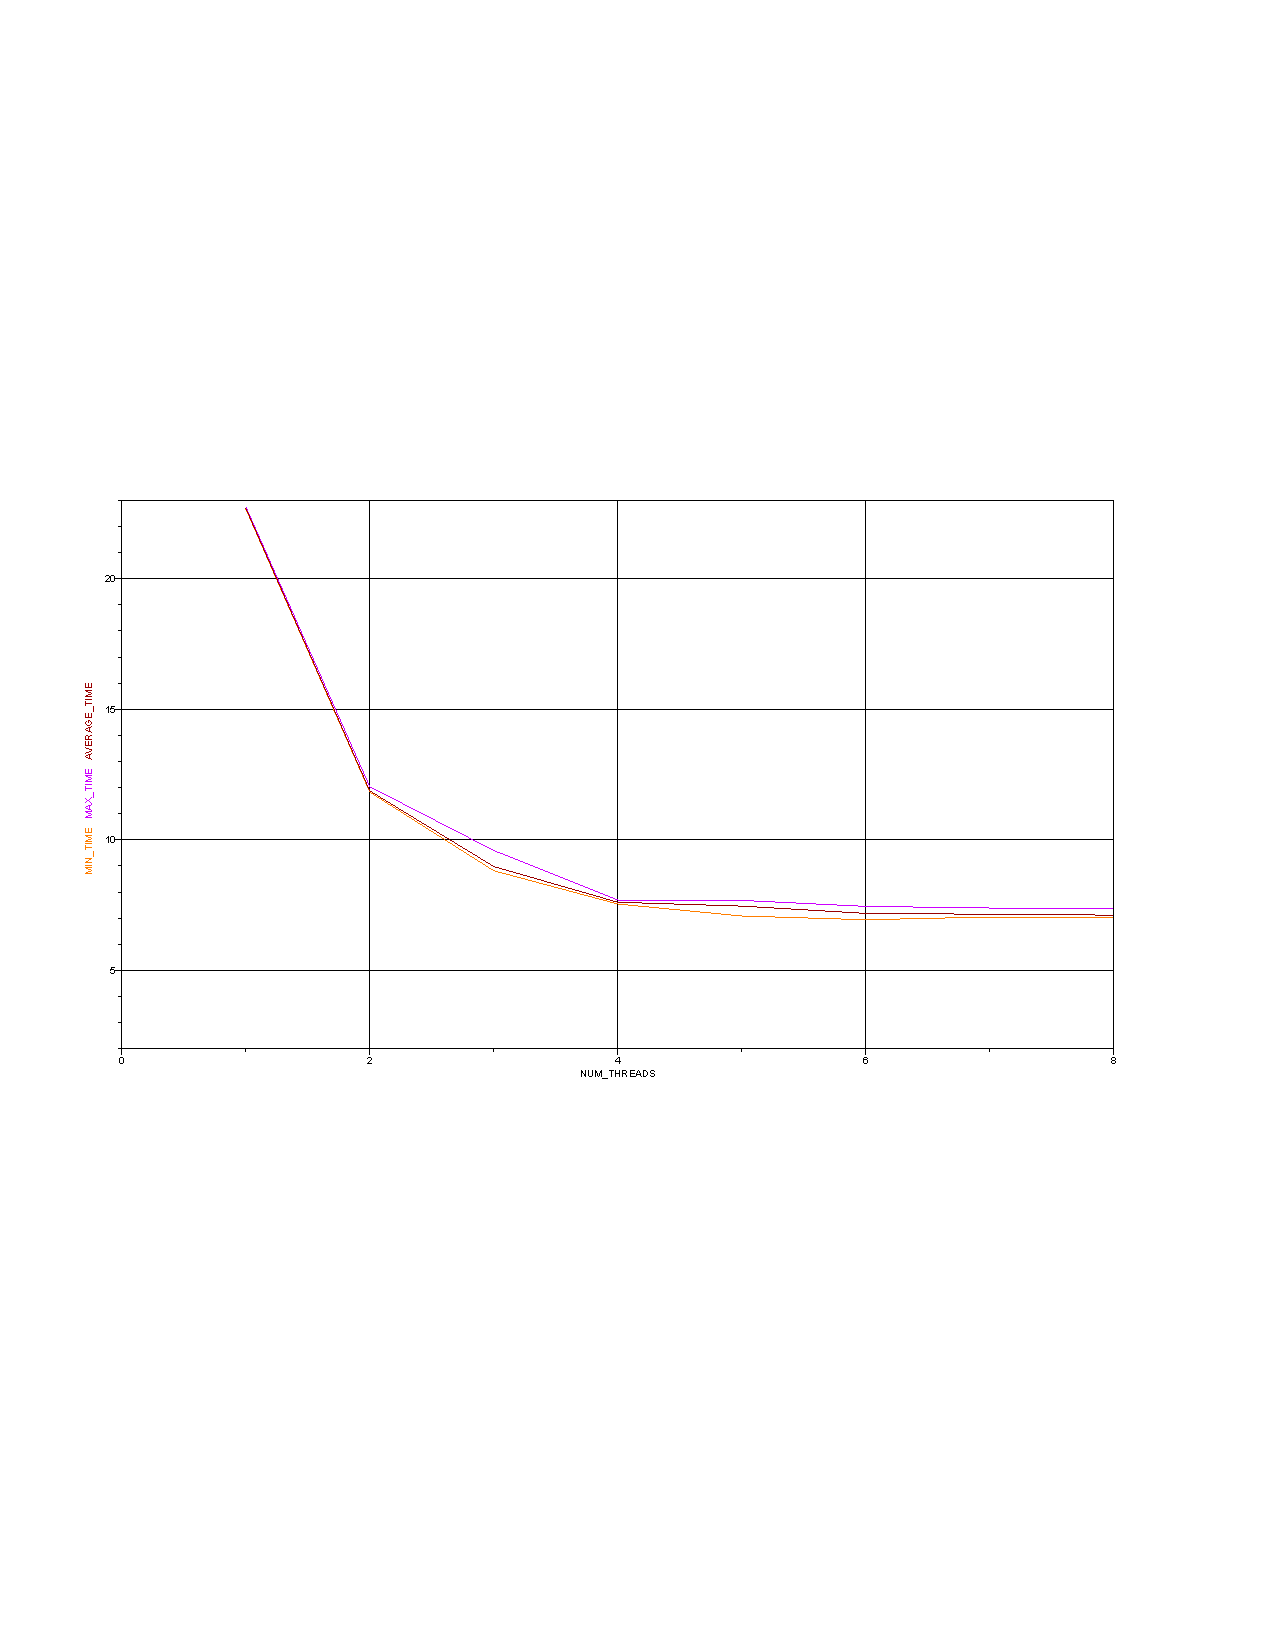
\includegraphics[scale=0.5]{images/pthread_time.pdf}
\subsubsection*{MPI Min/Max/Average Times per Thread}
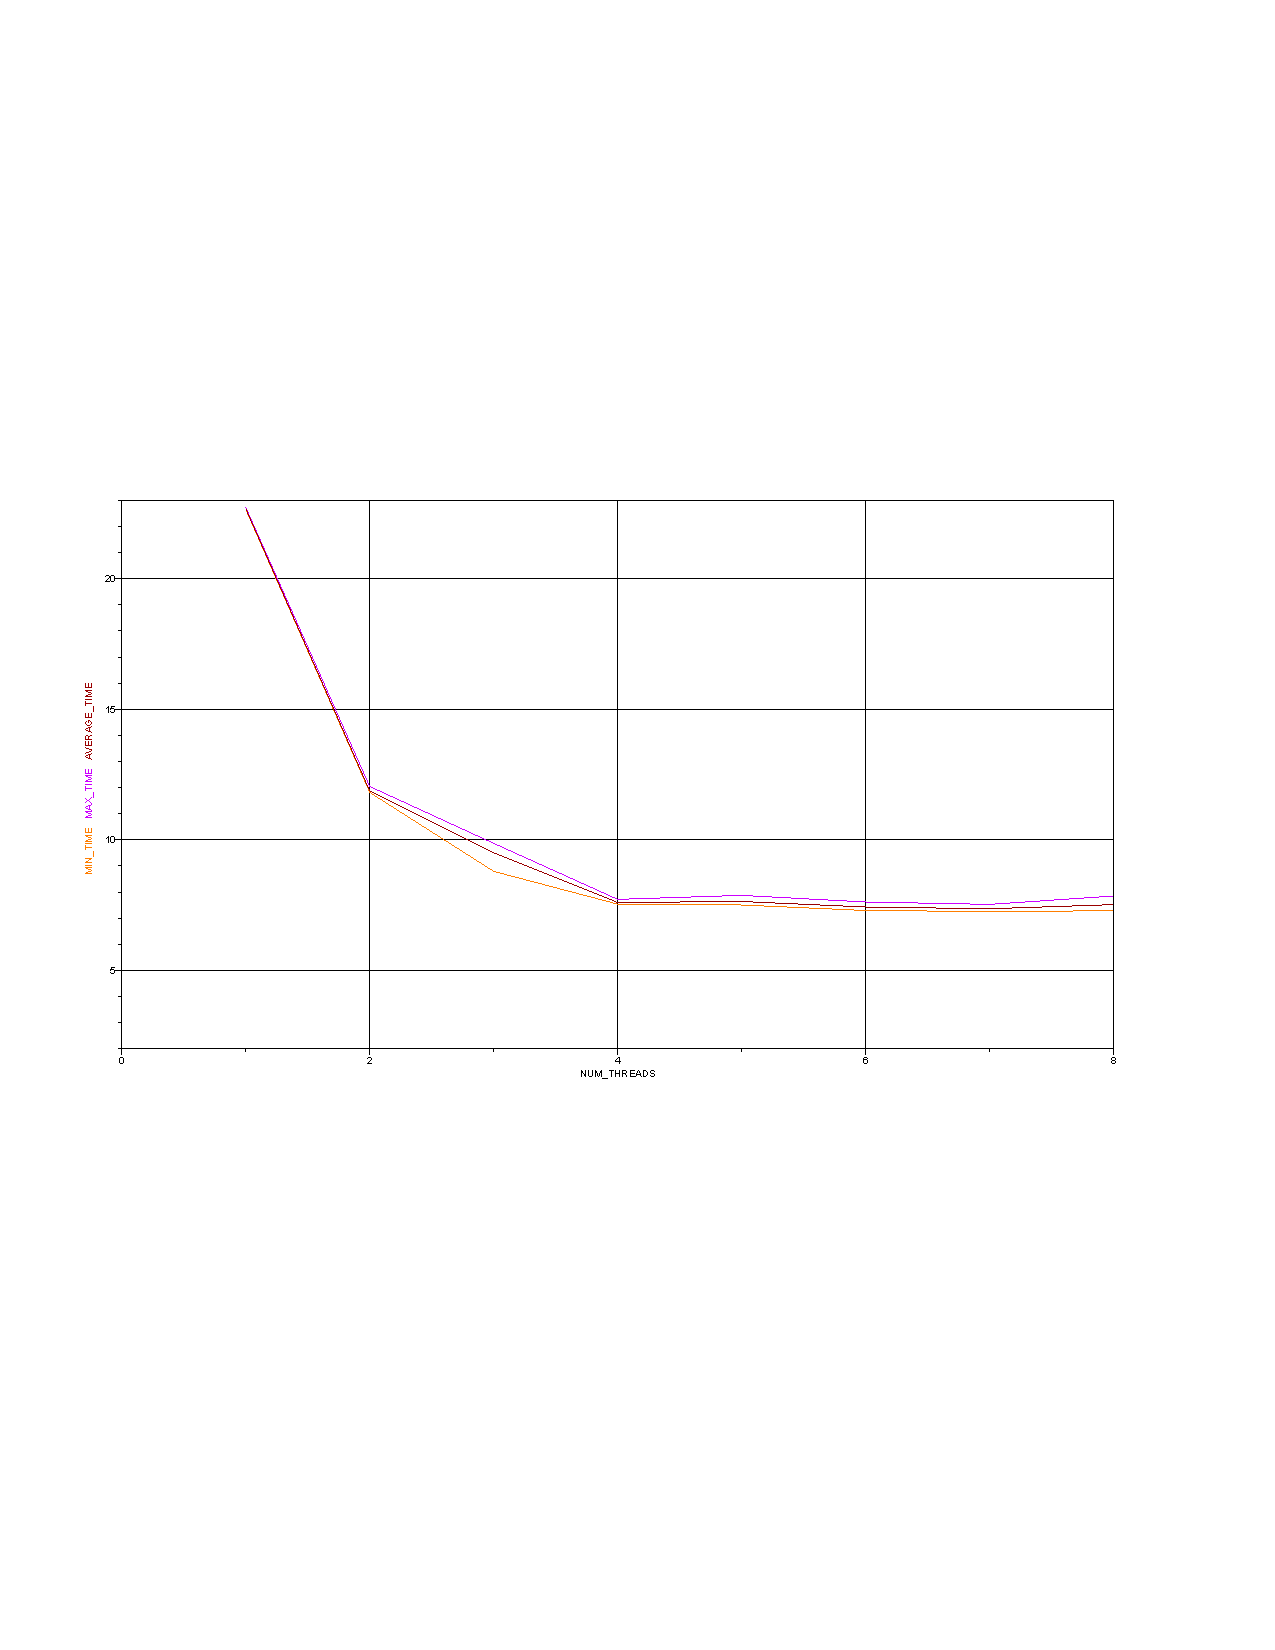
\includegraphics[scale=0.5]{images/mpi_times.pdf}\\
Above are more tiny graphs dedicated to showing the speedup over time, and the true inquiry in which I wanted to set out to answer. I attempted to measure the program as close to purely parallel as possible. It's difficult to ascertain exactly how much of my program is parallel especially since I don't know a lot of the intricacies of how much cpu work it takes to spin off threads and processes for these parallel methods, but we can conservatively state that we have a 90\% parallelized program.\\
$$v=\frac{1}{(1-P)+\frac{P}{S}}$$
Using Ahmdal's law with a 90\% assumption of speedup, we can utilize the values of when threads are equal to 1 (serial) to compare speedup to expected.
\subsection*{OpenMP}
\subsubsection*{Serial}
OpenMP with a single thread was able to perform the program in $22.699072$ seconds. This is our baseline.
\subsubsection*{2 Threads}
Based off of our Amdahl's law calculation, we should see a $1.81$ times speedup of this calculation -- which should be $12.54$ seconds.\\
Based off of my testing, the average time for two threads was $11.856366000000003$ seconds. This means that we saw a $1.91$ times speedup in our code. Based off of Amdahl's law, this means that our parallelized portion was actually closer to $95.5\%$ and I'll utilize future calculations based off of my new estimate.
\subsubsection*{3 Threads}
Based off of our new Amdahl's law figure, we should see a $2.75$ times increase in speed -- roughly $8.25$ seconds.\\
My average time came back as $9.516972999999998$ seconds, slightly above our new Amdahl's law figure. For the sake of comparison, and due to the increased workload of spinning off additional threads increasing our non-parallel sections, I'll assume for now that it is my original 90\%\\
This speedup is $2.39$ times that of our serial program.
\subsubsection*{4 Threads}
$7.5448119999999985$ seconds, a $3.01$ times speedup
\subsubsection*{5 Threads}
$7.419565999999999$ seconds, a $3.05$ times speedup
\subsubsection*{6 Threads}
$7.264279$ Seconds, a $3.12$ times speedup
\subsubsection*{7 Threads}
$7.204687$ Seconds, a $3.15$ times speedup
\subsubsection*{8 Threads}
$7.129125999999999$ seconds, a $3.18$ times speedup.
\subsection*{Pthread}
\subsubsection*{Serial}
$22.686887000000002$ seconds
\subsubsection*{2 Threads}
$11.871498999999998$ seconds, a $1.91$ times speedup
\subsubsection*{3 Threads}
$8.979035$ seconds, a $2.52$ times speedup
\subsubsection*{4 Threads}
$7.610709$ seconds, a $2.98$ times speedup
\subsubsection*{5 Threads}
$7.462929$ seconds, a $3.04$ times speedup
\subsubsection*{6 Threads}
$7.184908$ seconds, a $3.16$ times speedup
\subsubsection*{7 Threads}
$7.149879$ seconds, a $3.17$ times speedup
\subsubsection*{8 Threads}
$7.118075$ seconds, a $3.19$ times speedup
\subsection*{MPI}
\subsubsection*{Serial}
$22.667635$ seconds
\subsubsection*{2 Processes}
$11.864985999999998$ seconds, a $1.91$ times speedup.
\subsubsection*{3 Processes}
$9.506274$ seconds, a $2.38$ times speedup
\subsubsection*{4 Processes}
$7.598731000000001$ seconds, a $2.98$ times speedup
\subsubsection*{5 Processes}
$7.6394280000000006$ seconds, a $2.97$ times speedup
\subsubsection*{6 Processes}
$7.426807000000001$ seconds, a $3.05$ times speedup
\subsubsection*{7 Processes}
$7.361805000000001$ seconds, a $3.08$ times speedup
\subsubsection*{8 Processes}
$7.517698$ seconds, a $3.02$ times speedup
\subsection*{Conclusion On Timings}
The speedup that we were able to get by increasing the number of threads between 1, 2, 3, and 4, were nearly what we would assume. While I'm sure there is more to play than I'm assuming, plus this is a fully functioning OS handling other tasks in the background, we saw a steady and reliable increase in speedup between these thread counts/process counts. Because at 4 threads or processes, we have maxed out the number of cores that my system has, we no longer see a significant speedup, if at all in MPI's case. Instead, from 4-8 threads, we only see a minimal amount of speed up. Due to the extreme costs of adding additional thread testing to the suite (as this suite took roughly an hour to compute), I decided to sparsely test above 8 threads, but not report it verbosely. After the spinoff of 8 threads or processes, we actually start to see a small slowdown in performance accross the board. This is because my system is no longer able to keep up with the number of threads, and the overhead of more threads was too great to see any additional speedup. The same thought could have been had for adding 4-8 more threads, but the benefit still stands to add those for two reasons. First, my CPU is hyper threaded meaning that each core could potentially context switch between two threads at once causing a minor but noticeable speedup. Second, if, perhaps, a single thread gets done with it's tasks first, it doesn't necessarily have to sit in wait for the rest of the cores to be done. Smaller chunk sizes means that a beefier core would be able to do more work so that more of the CPU will be active during the program.
\subsection*{Comparing Methods}
Thread Counts. (OpenMP,Pthread,MPI) speedup:
\begin{enumerate}
	\item (1,1,1)
	\item (1.91,1.91,1.91)
	\item (2.39,2.52,2.38)
	\item (3.01,2.98,2.98)
	\item (3.05,3.04,2.97)
	\item (3.12,3.16,3.05)
	\item (3.15,3.17,3.08)
	\item (3.18,3.19,3.02)
\end{enumerate}
As can be seen, all three methods performed identically for one and two threads. At three threads, we can see that MPI and OpenMP did roughly the same, with pthreads taking a slight lead. Pthreads then fell behind OpenMP for 3 and 4 threads. I believe that this is due to someone much smarter than I am implementing OpenMP, while I'm still relatively new to pthreads. I fully expect that I should be able to get my pthread code consistently higher or the same as openmp code for most situations if I was an expert at it. MPI, of course since it doesn't have shared memory or benefit from hyperthreading falls behind after 2 threads only getting worse the more processes we added.
\subsubsection*{Conclusion}
Obviously if we are able to created a shared memory threaded processes, it will outperform the same program of a distributed memory process. But between Pthreads and OpenMP, the performance based off of my limited calculations seems to be roughly the same. Especially since this was an embarassingly parallelizable problem, I think that the logic held by OpenMP to automatically thread my program was sufficient enough to keep up, where a less parallelizable program would probably benefit more from the fine grained tuning that comes with Pthreads.
\subsection*{Hybrid System}
The extensiveness of the testing of my single method programs disallowed me from performing this on the cluster system available to me. As such, I was not capable of keeping the performance of the system(s) consistent across testing. As such, I have implemented the hybrid systems as more of a though experiment than a robust method of saying what is conclusively the best method.\\
As such, I ran two different systems -- one with 4 processes across 2, 2 core systems each processes running two threads of calculation. The average time I received for my OpenMP implementation was $5.362361$ seconds, with the Pthreaded version running at $5.236873000000001$ seconds on average accross 5 runs. This means that despite my laptop being consistently better than a single cluster node, the total of 8 threads running distributed over two systems containing a total of two cores somehow beat out my 8 threaded implementation.
\end{document}
